
\documentclass [a4paper] {article}
\usepackage[utf8]{inputenc}
\title{Ciencia de datos, práctica 1}
\author{Juan Casado Ballesteros}
\usepackage{Sweave}
\begin{document}
\maketitle

\begin{abstract}
En esta práctica vamos a realizar tres análisis estadísticos, 
en los dos primeros utilizaremos las funciones propias de R sobre los datos proporcionados por el profesor en los formatos .txt para el primero y .sav para el segundo.
En el tercer análisis hemos programado nosotros mismos nuestras propias funciones. 
Como datos hemos elegido un .csv que contiene información sobre el alquiler en la Ciudad de Nueva York.
Intentaremos para este tercer análisis realizar un estudio crítico que nos permita llegar a conocer los datos con los que estamos trabajando.

Las dos últimas secciones del documento hacen referencia a dos listados de funciones, 
el primero de las funciones de R que deberíamos conocer y el segundo de las creadas por nosotros junto a su implementación.
\end{abstract}

\newpage
\tableofcontents
\newpage


%-----------------------------------------------------------------------------------------------------------------------------------------------------------------------
\section{Primer análisis satelites menores de urano.txt}
%-----------------------------------------------------------------------------------------------------------------------------------------------------------------------

Comenzamos leyendo los datos del archivo .txt ya que dicho archivo lo hemos escrito con la sintaxis que read.table espera 
no tendremos que utilizar ningún parámetro adicional para configurar la lectura de los datos.
\begin{Schunk}
\begin{Sinput}
> satelites <- read.table("./satelites.txt")
\end{Sinput}
\end{Schunk}

\subsection{Frecuencias}
\subsubsection{Frecuencia Absoluta}
Primero calcularemos la frecuencia absoluta de los datos, que es el número de apariciones de cada uno de ellos.
Vemos que todos los valores aparecen solo una vez excepto 20 que está dos veces.

\begin{Schunk}
\begin{Sinput}
> frecuencia_absoluta<-table(satelites$radio)
\end{Sinput}
\end{Schunk}
\begin{center}
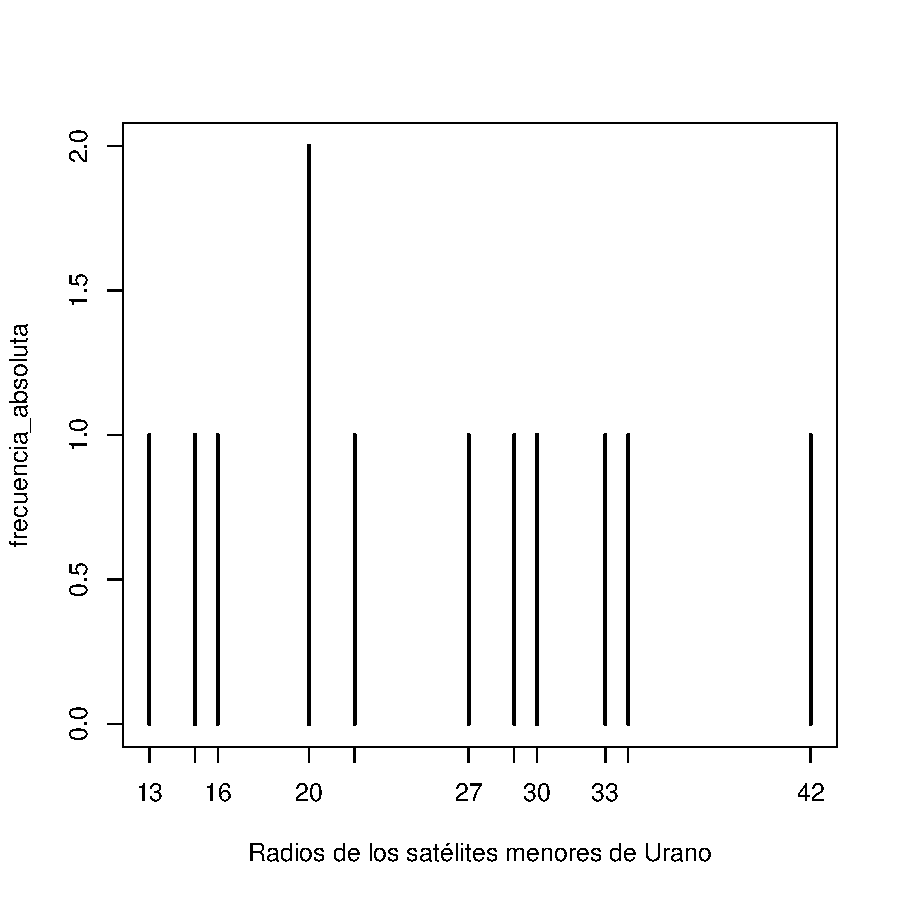
\includegraphics{entrega-frecuencia_absoluta_satelites_plot}
\end{center}

La moda es el dato cuya frecuencia absolutaes mayor.
\begin{Schunk}
\begin{Sinput}
> datos_ordenados=sort(frecuencia_absoluta,TRUE)
> moda_ <- as.numeric(rownames(as.matrix(datos_ordenados))[1])
> moda_
\end{Sinput}
\begin{Soutput}
[1] 20
\end{Soutput}
\end{Schunk}

\subsubsection{Frecuencia Absoluta Acumulada}
Ahora calcularemos la frecuencia absoluta acumulada que es la crecuencia absoluta de cada dato sumada con la de todos los menores a él.
La frecuencia absoluta se va incrementadndo de forma uniforme, de uno en uno, hasta llegar a 20 que aumenta en dos tal y comno se esperaba.

Cuando utilizamos la función textbf{cumsum}, cuya función es acumular las frecuencias, es recomendable aplicar as.table para que los datos sigan en el formato de tabla.
Esto nos permitirá luego mostrarlos en la gráfica sin problemas.

\begin{Schunk}
\begin{Sinput}
> frecuencia_absoluta_acumulada<-as.table(cumsum(frecuencia_absoluta))
\end{Sinput}
\end{Schunk}
\begin{center}
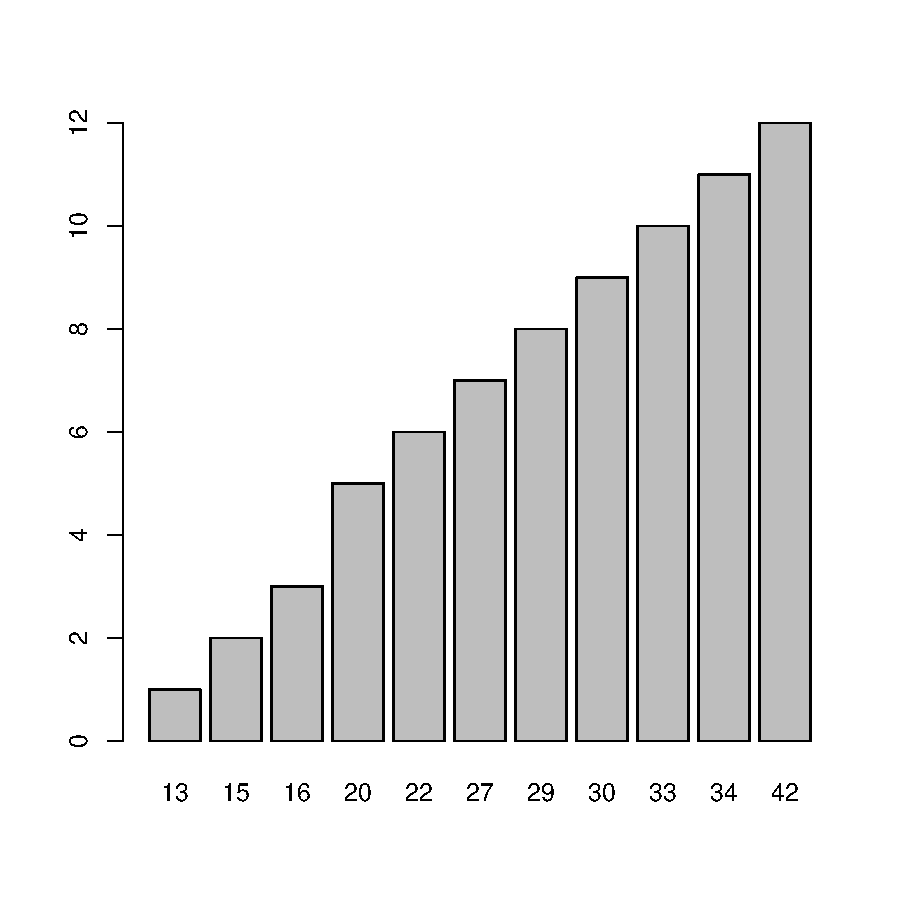
\includegraphics{entrega-frecuencia_absoluta_acumulada_satelites_plot}
\end{center}

\newpage
\subsubsection{Frecuencia Relativa}
La frecuencia relativa que es la frecuencia absoluta dividida por la cantidad de datos que hay.
La suma de las frecuencias relativas debe dar 1 como resultado lo cual comprobamos.
La frecuncia relativa por si sola aporta más información que la frecuencia absoluta pues está normalizada entre dos valores conocidos 0 y 1.
Para que la frecuencia absoluta nos aporte la misma información necesitamos conocer la cantidad de valores que tenemos para poder enmarcar el dato en su contexto.

\begin{Schunk}
\begin{Sinput}
> frecuencia_relativa <- (function(data) table(data)/length(data))(satelites$radio)
> sum(frecuencia_relativa)
\end{Sinput}
\begin{Soutput}
[1] 1
\end{Soutput}
\end{Schunk}
\begin{center}
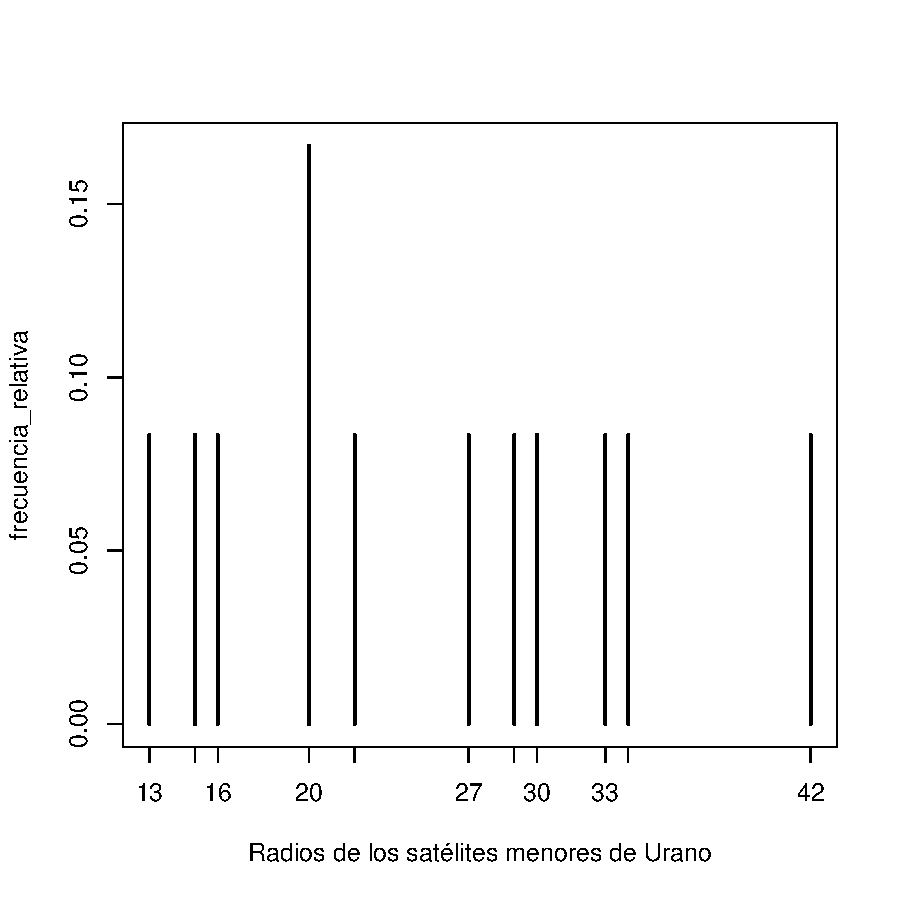
\includegraphics{entrega-frecuencia_relativa_satelites_plot}
\end{center}

\newpage
\subsubsection{Frecuencia Relativa Acumulada}
La frecuencia relativa acumulada que es la suma de la frecuencia relativa de cada valor con la de los menores a él.

\begin{Schunk}
\begin{Sinput}
> frecuencia_relativa_acumulada <- as.table(cumsum(frecuencia_relativa))
\end{Sinput}
\end{Schunk}
\begin{center}
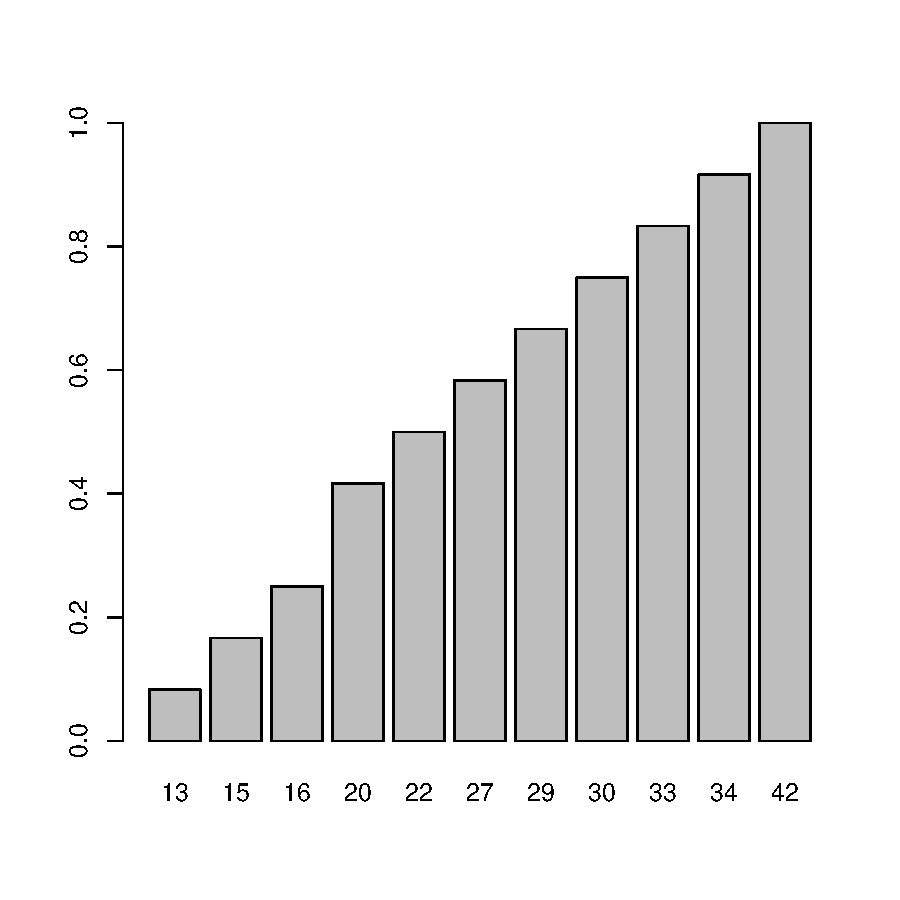
\includegraphics{entrega-frecuencia_relativa_acumulada_satelites_plot}
\end{center}

\newpage
\subsection{Valores representativos}
Calcularemos a continuación estadísticos cuya función es resumir los datos de los que disponemos.

\subsubsection{Media aritmética}
La media aritméticaconsite en una suma de los datos ponderada por la cantidad de estos.
Como podemos ver la media está ligeramente desplazada del centro del rango (29) siendo más próxima a radios de menor tamaño.

\begin{Schunk}
\begin{Sinput}
> media_ <- mean(satelites$radio)
> media_
\end{Sinput}
\begin{Soutput}
[1] 25.08333
\end{Soutput}
\end{Schunk}

\subsubsection{Desviación típica}
La desviacion típica es pequeña lo que hace que la media sea una buen valor para representar a los datos.
Sabemos que la media es buena a partir de la desviacion típica obtenida utilizando el teorema de tchebychev vemos 
que los valores de todos los radios se los satélites quedan dentro del intervalo $[media-2 * desviación típica, media+2 * desviación típica]$ 
cuando como mínimo solo tendrían que estar el 75\%.

\begin{Schunk}
\begin{Sinput}
> desviacion_tipica_ <- sd(satelites$radio)
> desviacion_tipica_
\end{Sinput}
\begin{Soutput}
[1] 8.857029
\end{Soutput}
\end{Schunk}

Tchebychev para k=2, al menos el 75\% de los datos estarán dentro del rango $[media -2 * desviación típica, media +2 * desviación típica]$, 
para nuestro caso todos lo están.
\begin{Schunk}
\begin{Sinput}
> c(media_-2*desviacion_tipica_, media_+2*desviacion_tipica_)
\end{Sinput}
\begin{Soutput}
[1]  7.369275 42.797392
\end{Soutput}
\begin{Sinput}
> c(min(satelites$radio), max(satelites$radio))
\end{Sinput}
\begin{Soutput}
[1] 13 42
\end{Soutput}
\end{Schunk}

\subsubsection{Varianza}
La varianza es el cuadrado de la desviación típica.

\begin{Schunk}
\begin{Sinput}
> varianza_ <- var(satelites$radio)
> varianza_
\end{Sinput}
\begin{Soutput}
[1] 78.44697
\end{Soutput}
\end{Schunk}

\newpage
\subsection{Medidas de ordenanción}
\subsubsection{Cuartiles}

Los cuartiles son aquellos valores de modo que si los ordenáramos sobre un vector estarían en los índices situados en el 25, 50 y 75\%.
Hemos podico comprobar que R para calcular los cuartiles no lo hace exáctamente así si no que utiliza una distribución de probabilidad.
Cuando calculamos los cuartiles a mano con las fómulas de clase obtendremos valores distintos.

La mediana es el valor que está justo en el centro de los valores ordenados, segundo cuartil.
\begin{Schunk}
\begin{Sinput}
> cuartiles_ <- quantile(satelites$radio, prob=c(0, .25, .5, .75, 1))
> cuartiles_
\end{Sinput}
\begin{Soutput}
   0%   25%   50%   75%  100% 
13.00 19.00 24.50 30.75 42.00 
\end{Soutput}
\begin{Sinput}
> mediana_ <- median(satelites$radio) #cuartiles_[2]
> mediana_
\end{Sinput}
\begin{Soutput}
[1] 24.5
\end{Soutput}
\end{Schunk}

\begin{center}
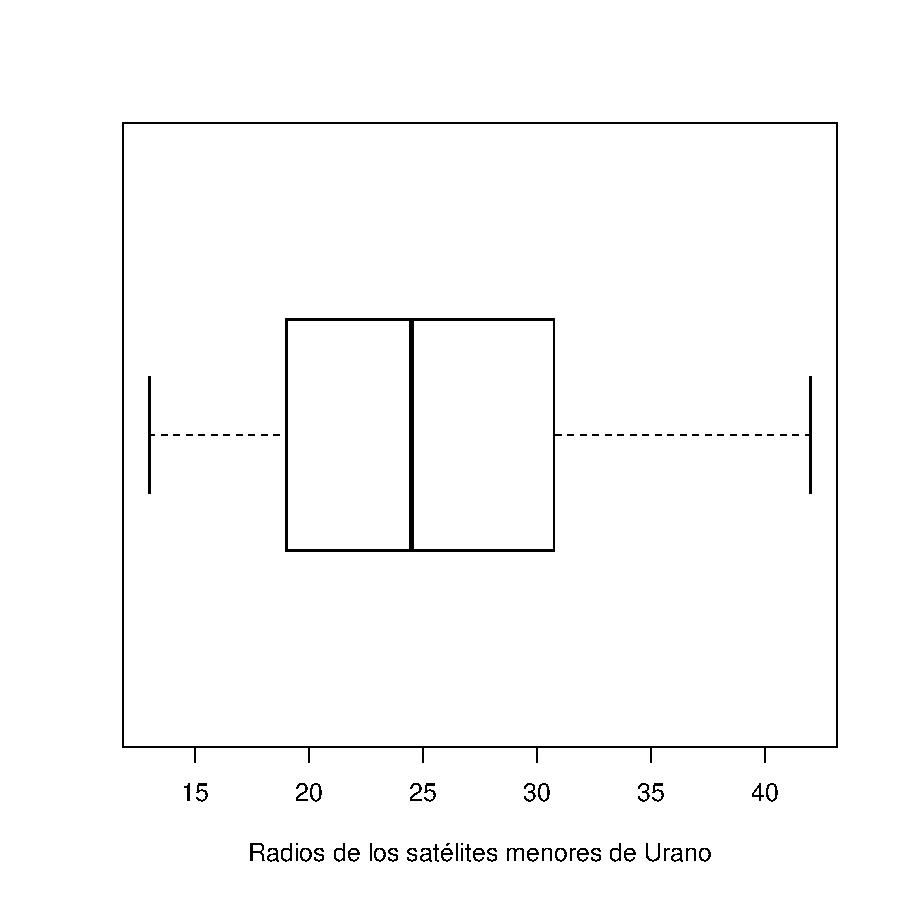
\includegraphics{entrega-cuartiles_satelites_plot}
\end{center}

\subsubsection{Cuartil 54}
\begin{Schunk}
\begin{Sinput}
> cuantil54_ <- quantile(satelites$radio, prob=(.54))
> cuantil54_
\end{Sinput}
\begin{Soutput}
 54% 
26.7 
\end{Soutput}
\end{Schunk}

\subsection{Visualización}
Hemos encontrado de gran utilidad representar sobre una misma gráfica la frecuencia relativa, la media, la moda y la mediana.
Esta representación proporciona la mayoría de la información estadística que estamos calculando de un solo vistazo y ayuda a entender como se
distrubuyen los datos que manejamos y cómo se relacionan con los valores que pretenden representarlos.
\begin{center}
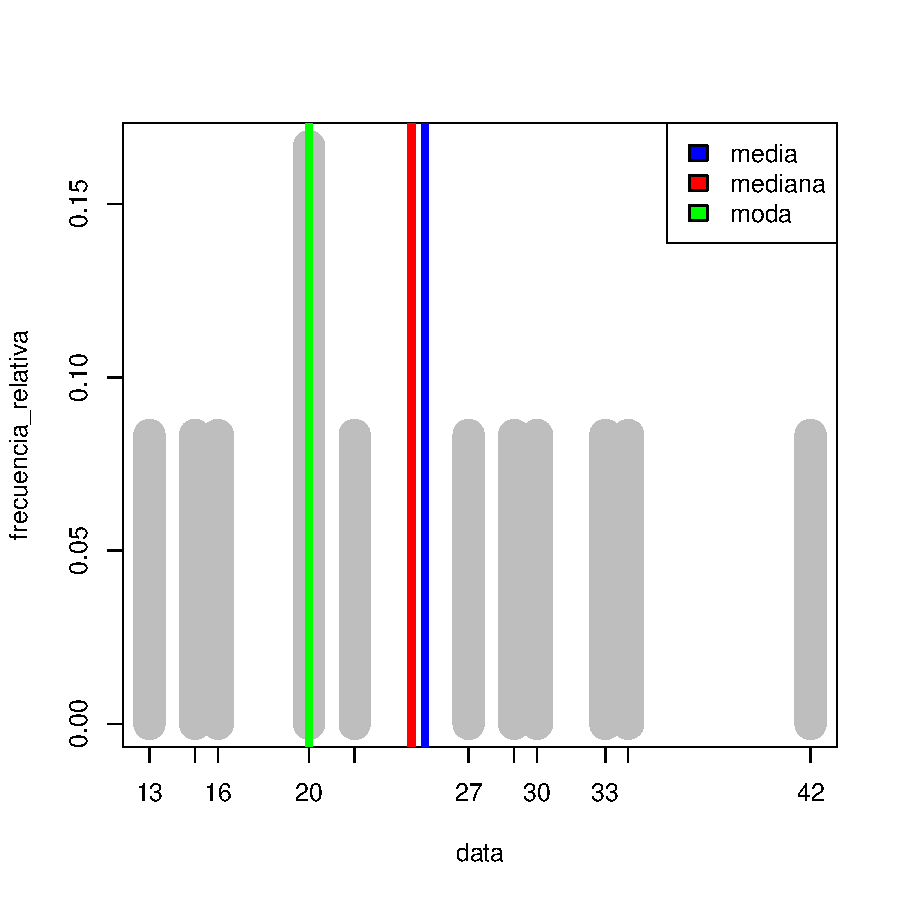
\includegraphics{entrega-estadisticos_satelites_plot}
\end{center}

\newpage
%-----------------------------------------------------------------------------------------------------------------------------------------------------------------------
\section{Segundo análisis cardata .sav}
%-----------------------------------------------------------------------------------------------------------------------------------------------------------------------

Para el segundo análisis estudiaremos los datos de la variable mpg que representa el consumo en millas por galón de un conjunto de automóbiles.
Comenzamos cargado los datos que deben ser preparados. 
Primero eliminamos el warning de Duplicated levels in factor y posteriormente eliminamos los valores nulos para poder realizar las operaciones correctamente.
\begin{Schunk}
\begin{Sinput}
> cardata <- read.spss("./cardata.sav", use.value.labels = FALSE)$mpg
> cardata <- cardata[!is.na(cardata)]
\end{Sinput}
\end{Schunk}

\subsection{Valores representativos}
\subsubsection{Media aritmética}
La media está muy próxima a la mediana (28.9) que a su ver está muy próxima al punto medio del rango de valores (31).
Podemos ver que está ligeramente desplazada hacia los valores menores sobre todo teniendo en cuenta que la moda es bastante elevada 
aunque esta muy poco representativa pues en general los valores se distribuyen de forma uniforme sobre el rango.
\begin{Schunk}
\begin{Sinput}
> mean(cardata)
\end{Sinput}
\begin{Soutput}
[1] 28.79351
\end{Soutput}
\end{Schunk}

\subsubsection{Desviación típica y varianza}
La desviación típica es baja, el radio de 2\*desviación típica del teorema de tchebychev cubre a gran parte de los valores, desde luego a más del 75\%.
Podemos decir que la media representa bien a los valores a pesar de que los que están en el extremo superior del rango queden un poco alejados de ella.
\begin{Schunk}
\begin{Sinput}
> sd(cardata)
\end{Sinput}
\begin{Soutput}
[1] 7.37721
\end{Soutput}
\begin{Sinput}
> var(cardata)
\end{Sinput}
\begin{Soutput}
[1] 54.42323
\end{Soutput}
\end{Schunk}

\begin{center}
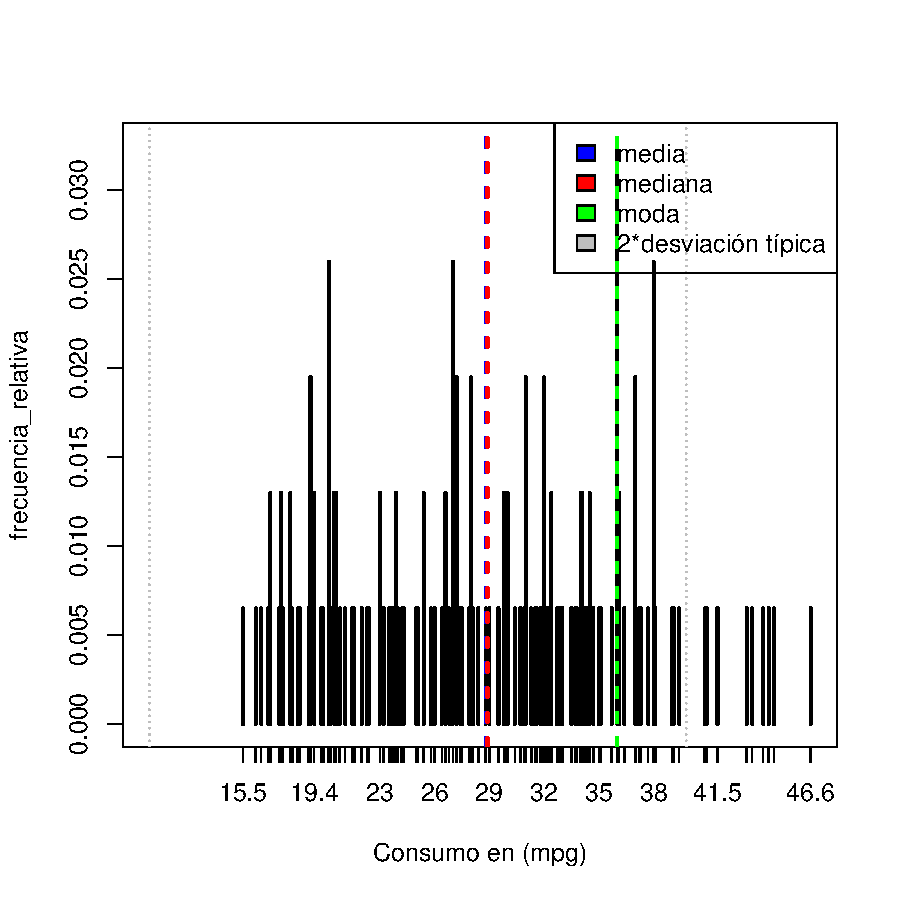
\includegraphics{entrega-estadisticos_cardata_plot}
\end{center}

\newpage
\subsection{Medidas de ordenanción}
Podemos ver como los datos están repartidos de una forma bastante homogénea a lo largo de su rango de valores.
\begin{Schunk}
\begin{Sinput}
> cuartiles_ <- quantile(cardata, prob=c(0, .25, .5, .75, 1))
> cuartiles_
\end{Sinput}
\begin{Soutput}
    0%    25%    50%    75%   100% 
15.500 22.550 28.900 34.275 46.600 
\end{Soutput}
\begin{Sinput}
> median(cardata) #cuartiles_[2]
\end{Sinput}
\begin{Soutput}
[1] 28.9
\end{Soutput}
\end{Schunk}
\begin{center}
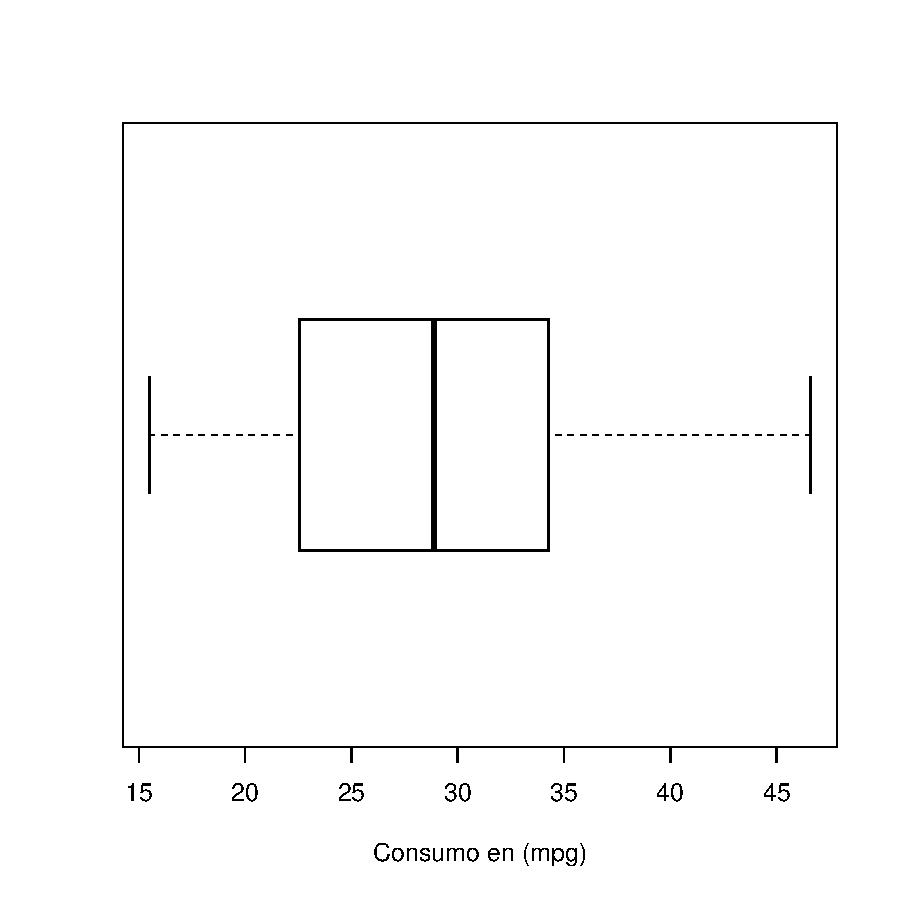
\includegraphics{entrega-ordenacion_cardata_plot}
\end{center}

\newpage
%-----------------------------------------------------------------------------------------------------------------------------------------------------------------------
\section{Tercer análisis del alquiler en Nueva York con AirBNB durante 2019 .csv}
%-----------------------------------------------------------------------------------------------------------------------------------------------------------------------

\begin{Schunk}
\begin{Sinput}
> data <- read.csv("AB_NYC_2019.csv") #https://www.kaggle.com/dgomonov/new-york-city-airbnb-open-data#AB_NYC_2019.csv
\end{Sinput}
\end{Schunk}

Haremos ahora un análisis de los datos del alquiler en la ciudad de Nueva York durante el año 2019 con la compañía AirBNB.
Los datos contienen las siguientes categorías:
\begin{Schunk}
\begin{Sinput}
> getInfo(data)
\end{Sinput}
\begin{Soutput}
                               unlist.res.
id                                 integer
name                                factor
host_id                            integer
host_name                           factor
neighbourhood_group                 factor
neighbourhood                       factor
latitude                           numeric
longitude                          numeric
room_type                           factor
price                              integer
minimum_nights                     integer
number_of_reviews                  integer
last_review                         factor
reviews_per_month                  numeric
calculated_host_listings_count     integer
availability_365                   integer
res_frame
 factor integer numeric 
      6       7       3 
\end{Soutput}
\end{Schunk}
Comenzaremos por analizar el precio de los alquileres.
Para ello calcularemos la frecuencia relativa de los precios.
\begin{Schunk}
\begin{Sinput}
> frecuencia_relativa<-frecuenciaAbsoluta(data$price)
\end{Sinput}
\end{Schunk}
\begin{center}
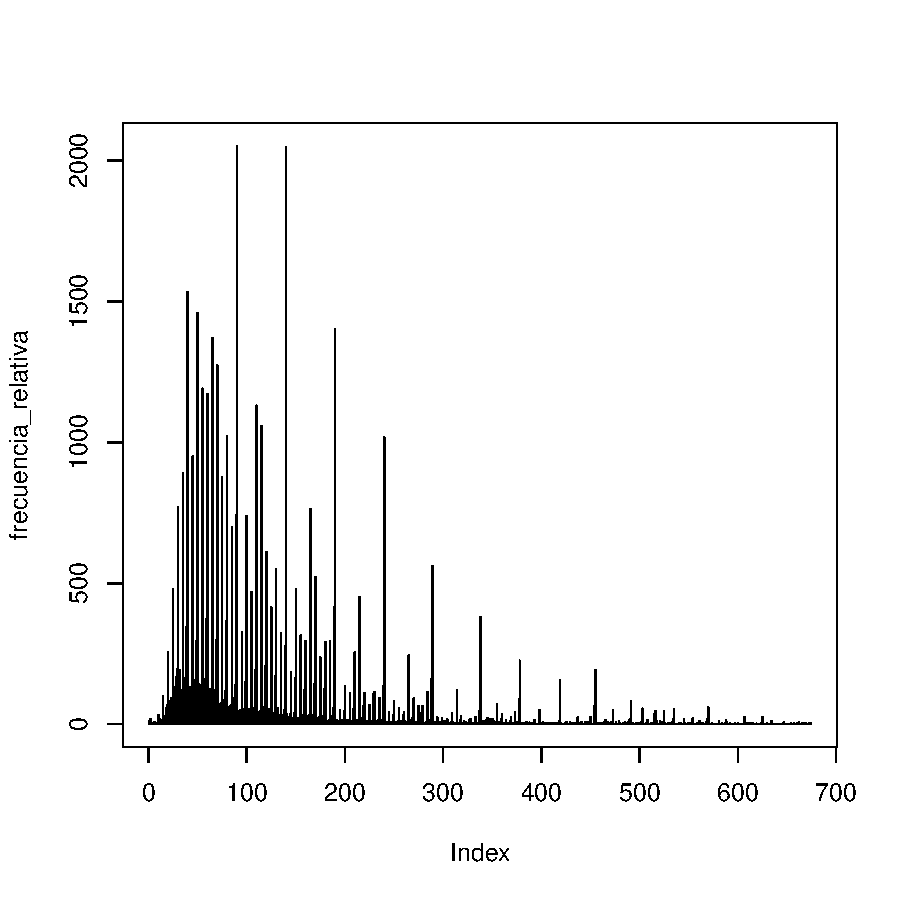
\includegraphics{entrega-frecuencia_relativa_BNB_plot}
\end{center}

Podemos observar que los precios están muy agrupados en la parte izquierda de la gráfica (precios bajos) con altos porcentajes de aparición,
no obstante aunque con una densidad mucho menor estos se alejan en gran medida llegando a alcanzar precios muy elevados pero con pocos porcentajes de aparición.

\begin{center}
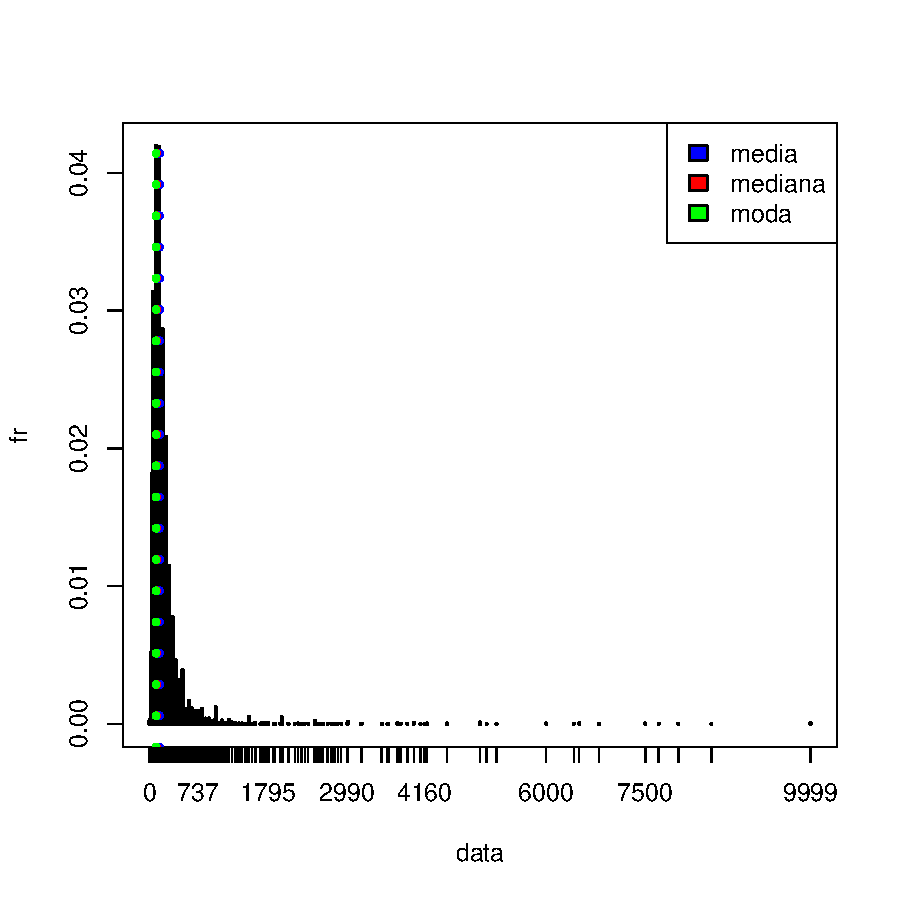
\includegraphics{entrega-estadisticos_BNB_plot}
\end{center}

\begin{Schunk}
\begin{Sinput}
> v_cuartiles <- cuartiles(data$price)
\end{Sinput}
\end{Schunk}
\begin{center}
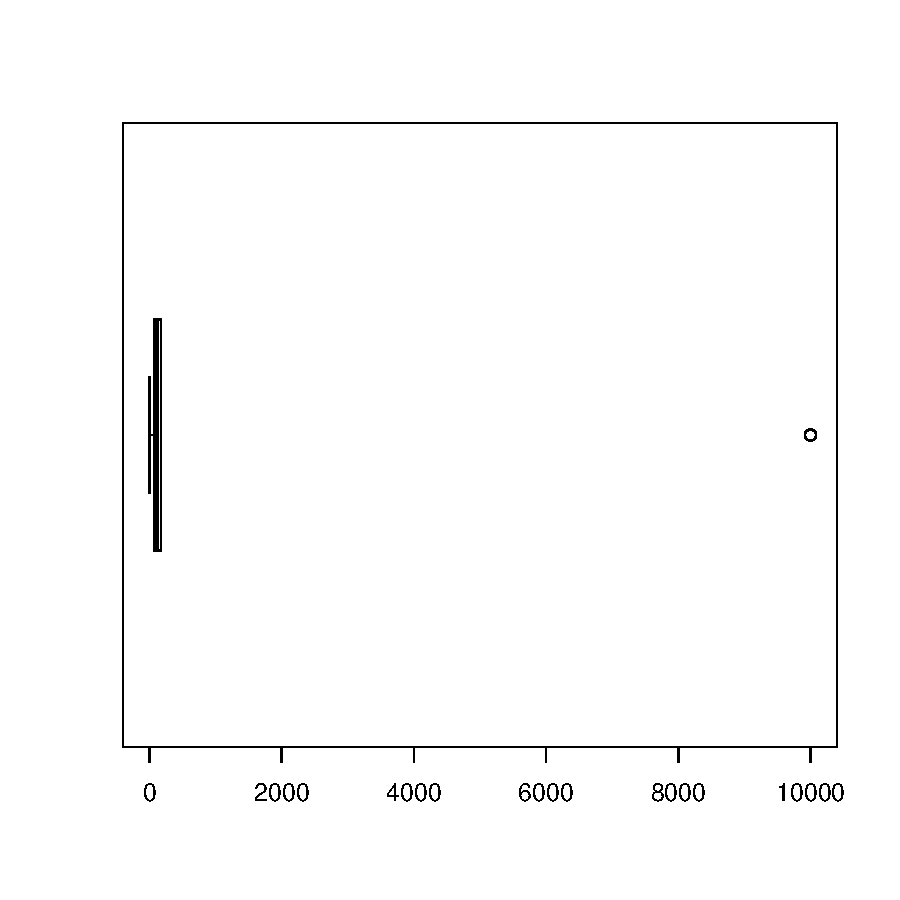
\includegraphics{entrega-cuartiles_BNB_plot}
\end{center}

Vemos que la media no es un valor representativo, su desviación típica es muy alta.
Podemos observar como la moda y la mediana en este caso parecen representar mejor a la mayoría de los datos.
Debido a esto decidimos que hacer el análisis de los precios para toda la ciudad no iba a aportarnos una visión representativa de los datos.
Decidimos ahora calcular el precio medio por cada barrio en vez de hacerlo sobre toda la ciudad a la vez.

\begin{Schunk}
\begin{Soutput}
        Group.1   x.media x.desviacion_tipica x.mediana    x.moda
1         Bronx  87.49679           106.66043  65.00000  60.00000
2      Brooklyn 124.38321           186.86889  90.00000 100.00000
3     Manhattan 196.87581           291.37646 150.00000 150.00000
4        Queens  99.51765           167.08741  75.00000  50.00000
5 Staten Island 114.81233           277.24801  75.00000  75.00000
\end{Soutput}
\end{Schunk}
Valores sobre el total de los datos sin haber separado por barrios
\begin{Schunk}
\begin{Soutput}
            media desviacion_tipica         v_mediana            v_moda 
         152.7207          240.1517          106.0000          100.0000 
\end{Soutput}
\end{Schunk}

Podemos ver que la varianza se ha reducido para más barrios de en los que ha aumentado.
En Bronx es en el barrio en el que tanto la varianza como la media es menor y 
Manhattan es en el que ambas son mayores.

Datos para Manhattan
\begin{center}
\begin{Schunk}
\begin{Sinput}
> manhattan_data = data$price[data$neighbourhood_group == "Manhattan"]
> plotFrecuencyData(manhattan_data)
\end{Sinput}
\end{Schunk}
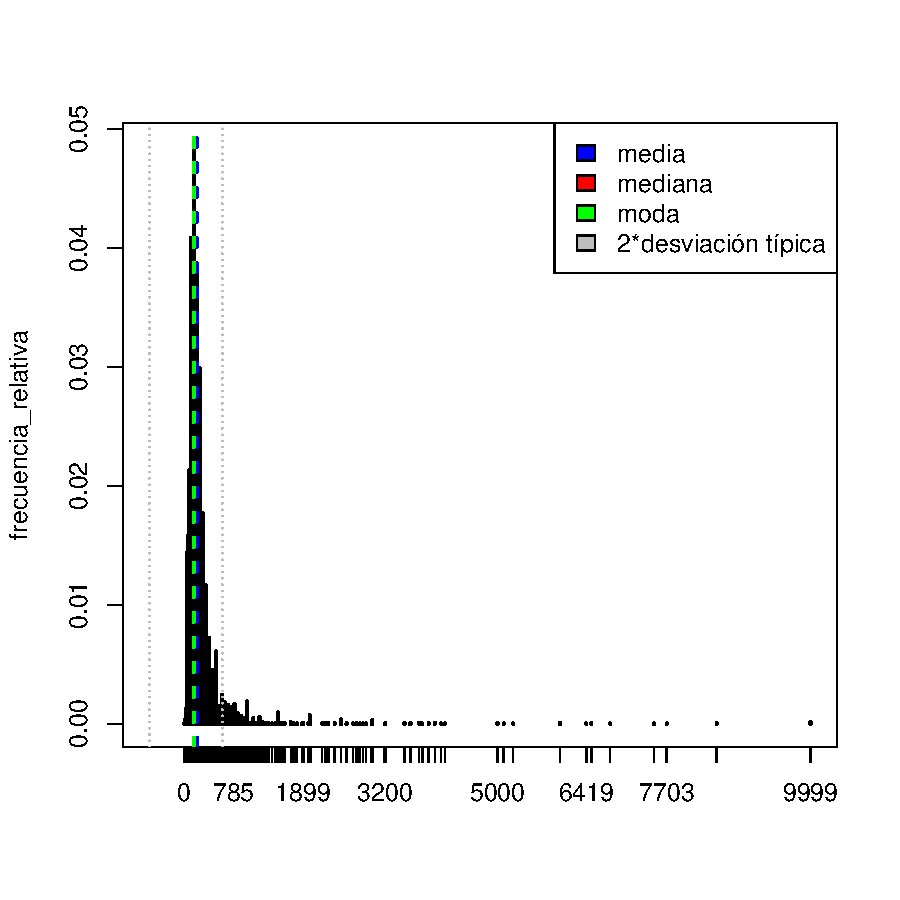
\includegraphics{entrega-035}
\end{center}
\begin{center}
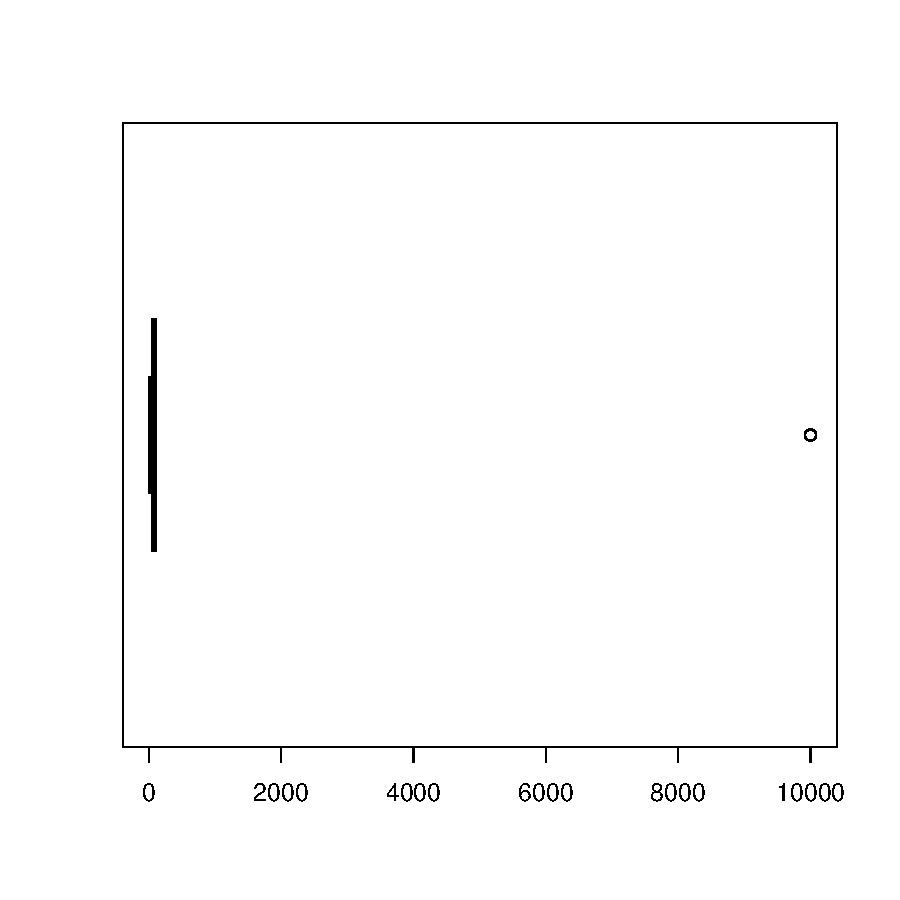
\includegraphics{entrega-036}
\end{center}

Datos para Bronx
\begin{center}
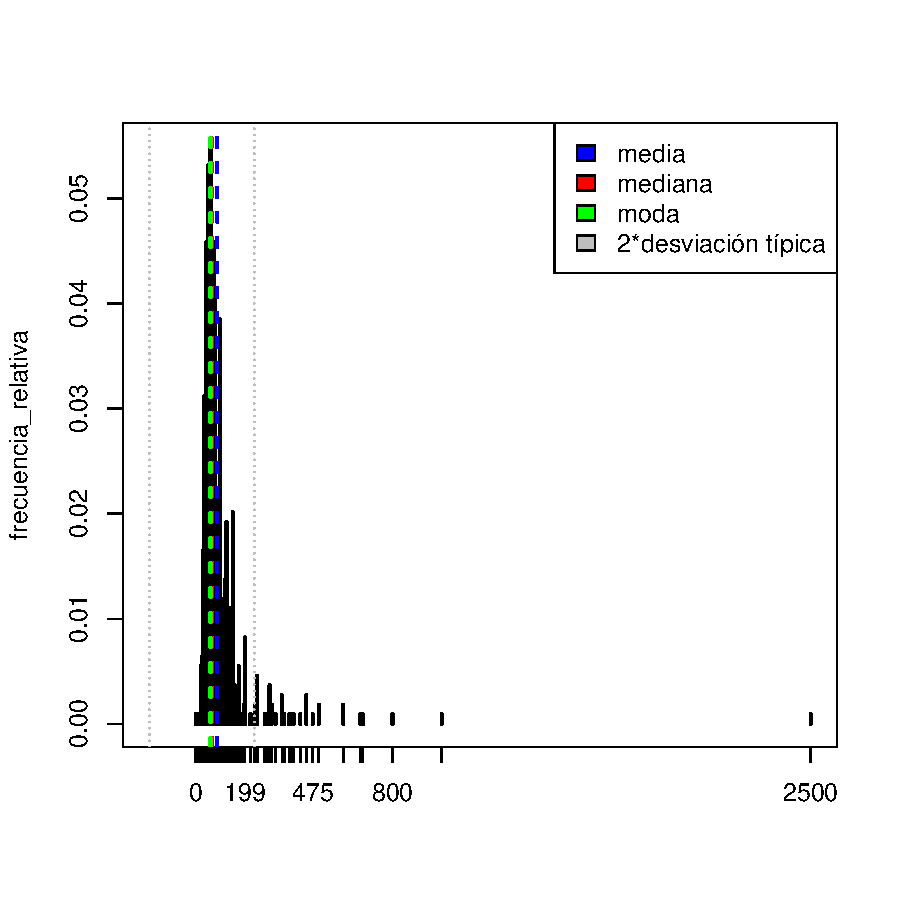
\includegraphics{entrega-037}
\end{center}
\begin{center}
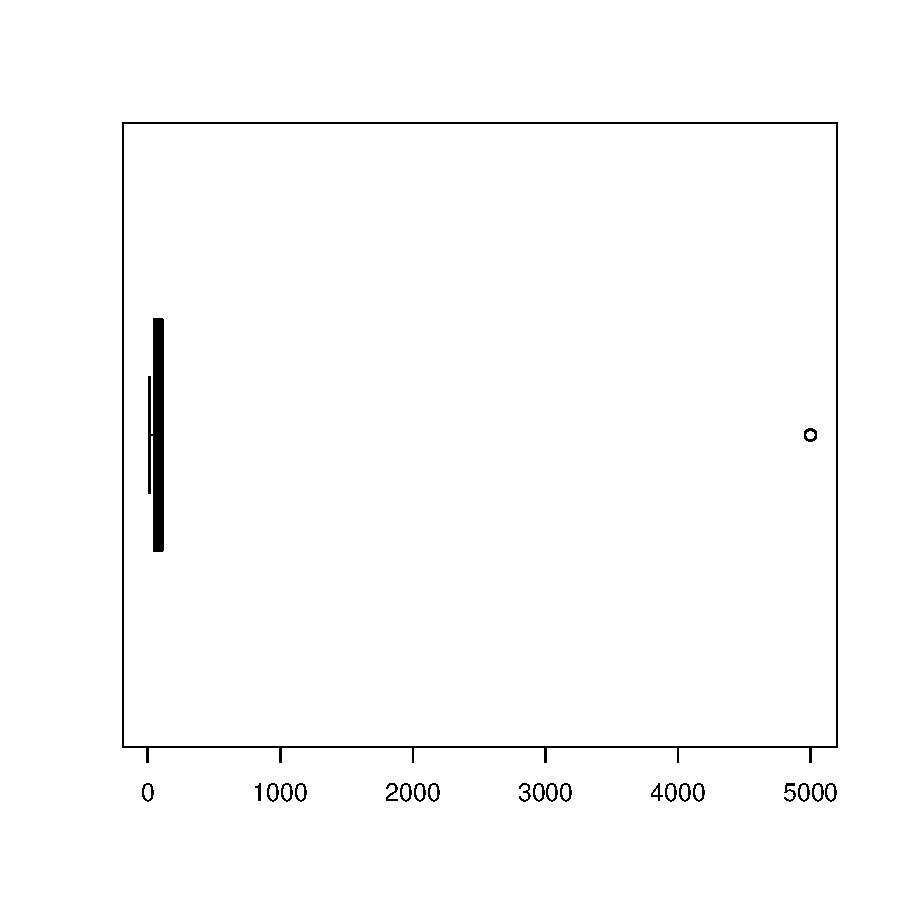
\includegraphics{entrega-038}
\end{center}

Datos para Brooklyn
\begin{center}
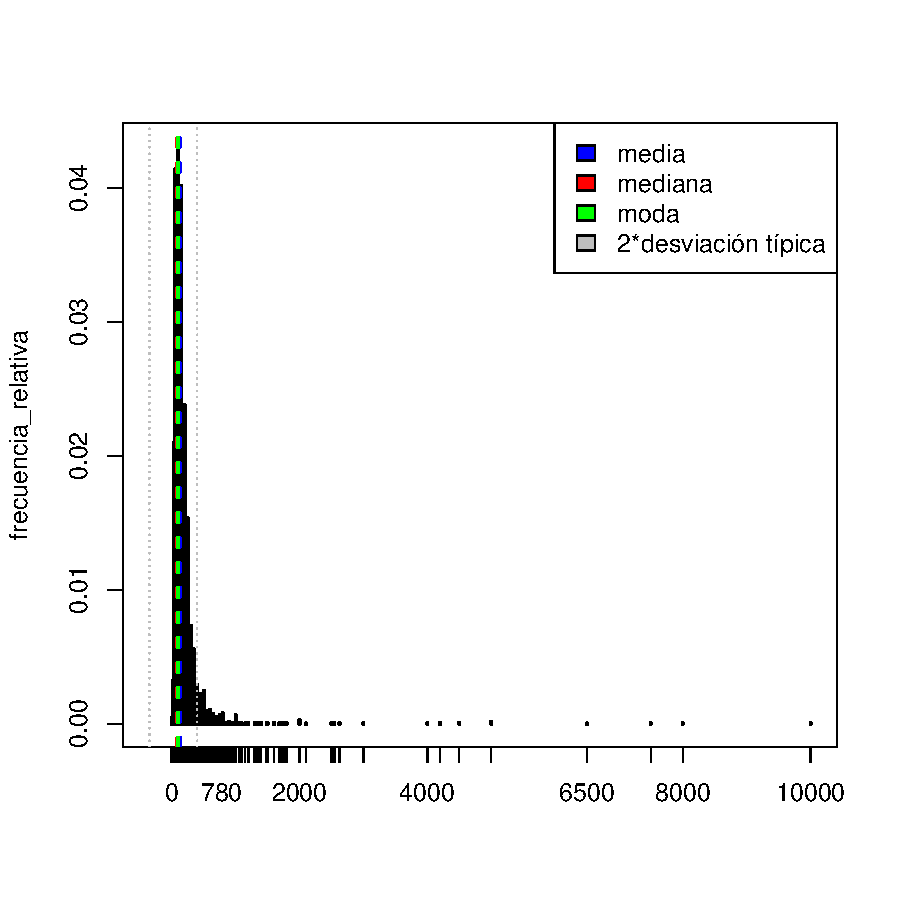
\includegraphics{entrega-039}
\end{center}
\begin{center}
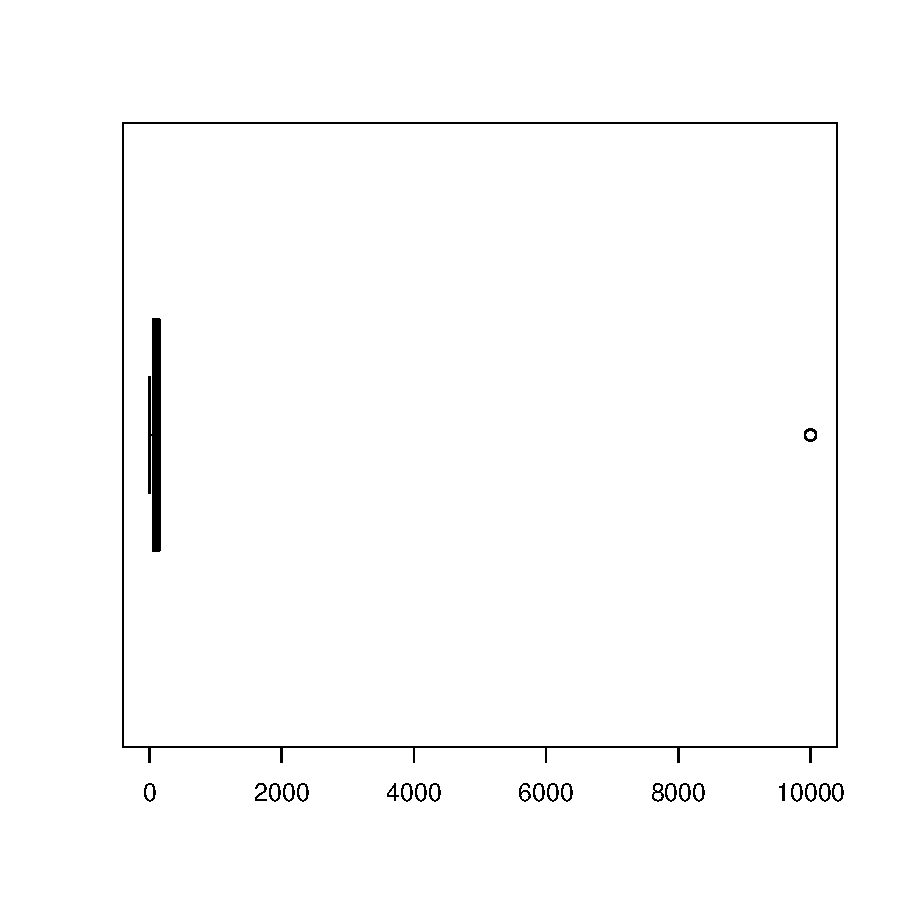
\includegraphics{entrega-040}
\end{center}

Datos para Queens
\begin{center}
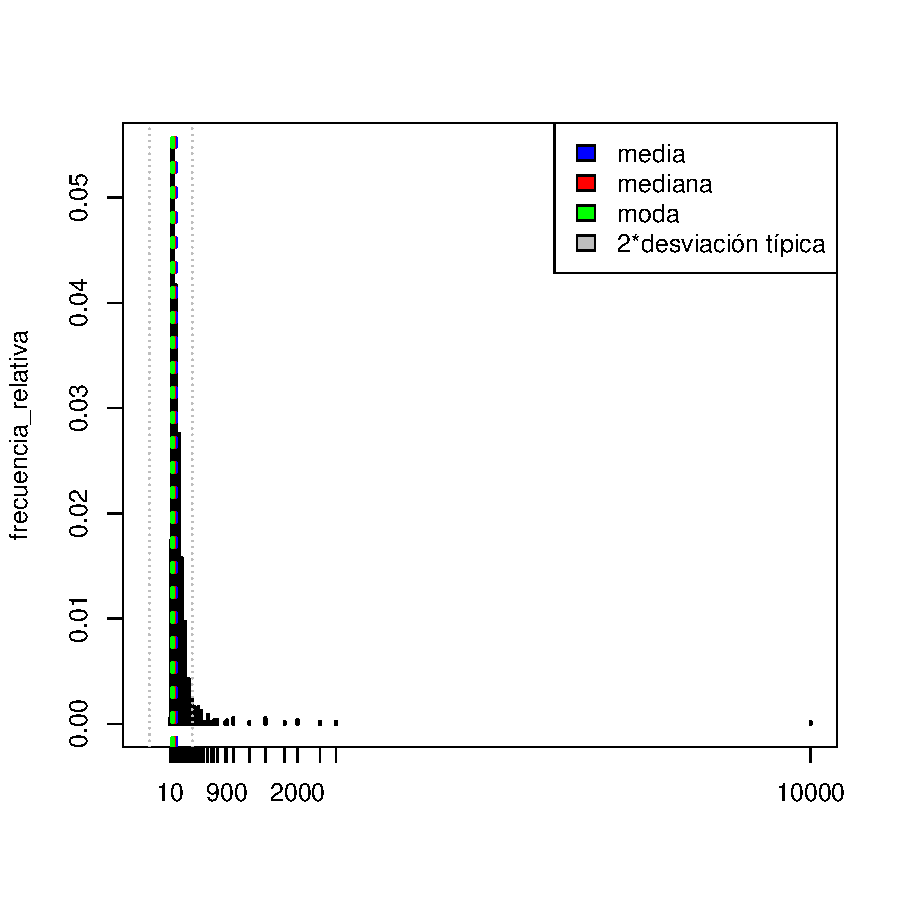
\includegraphics{entrega-041}
\end{center}
\begin{center}
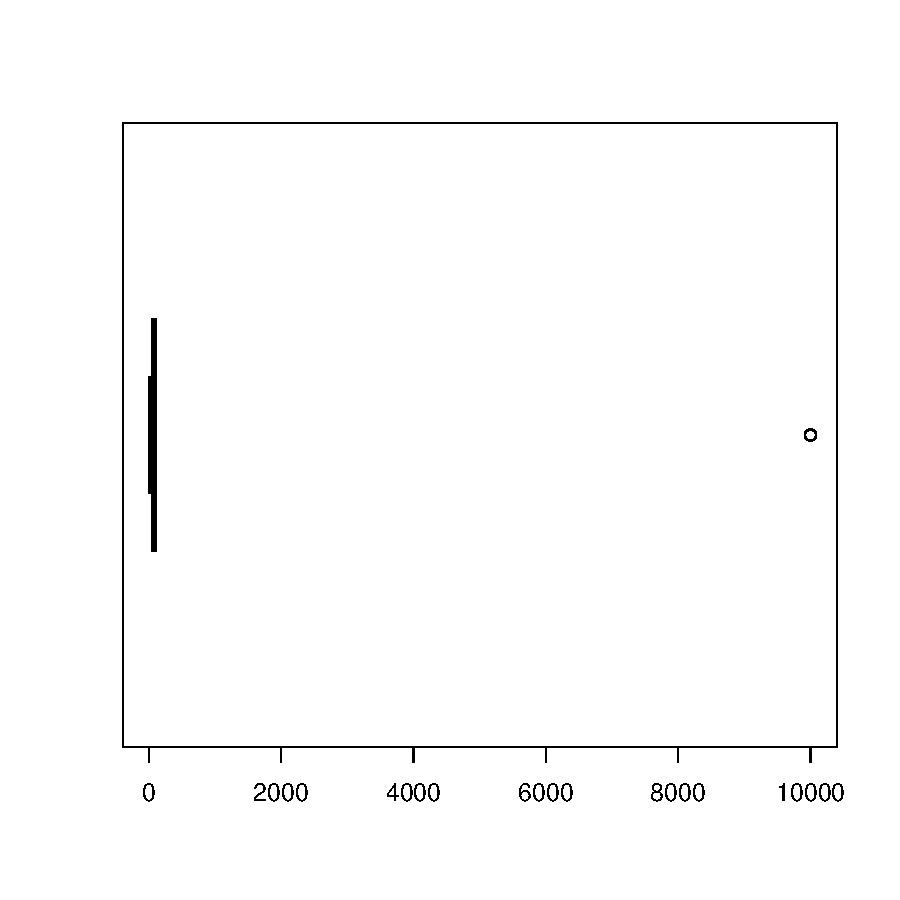
\includegraphics{entrega-042}
\end{center}

Datos para Staten Island
\begin{center}
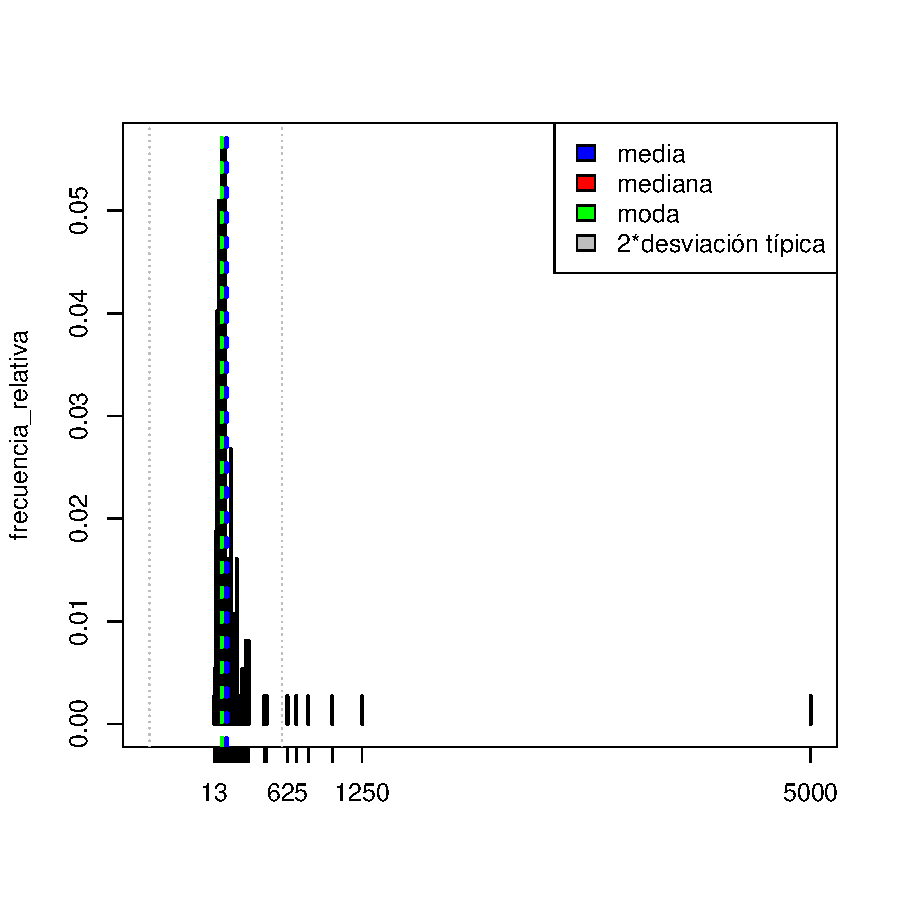
\includegraphics{entrega-043}
\end{center}
\begin{center}
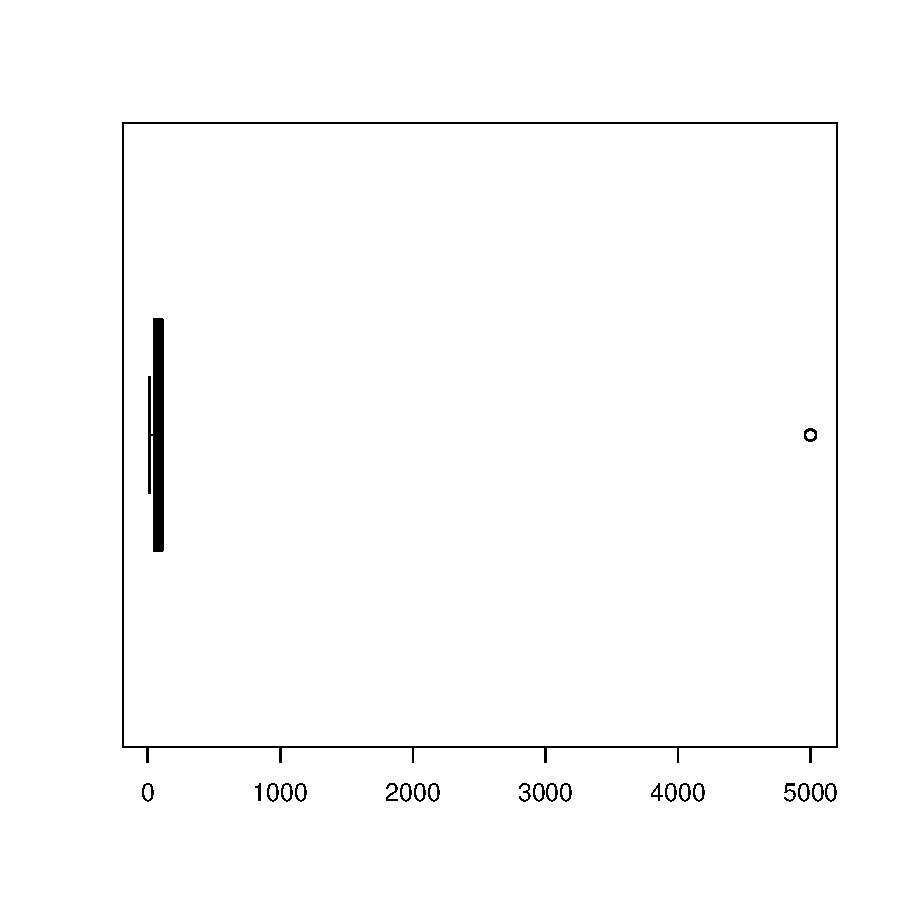
\includegraphics{entrega-044}
\end{center}
%-----------------------------------------------------------------------------------------------------------------------------------------------------------------------
\section{Guia en R para el análisis estadístico}
%-----------------------------------------------------------------------------------------------------------------------------------------------------------------------
\subsection{Frecuencias}
\begin{Schunk}
\begin{Sinput}
> Frecuencia_absoluta <- table(data)
> Frecuencia_absoluta_acumulada <- cumsum(frecuencia_absoluta)
> Frecuencia_relativa <- (function(data) table(data)/length(data))(data)
> Frecuencia_relativa_acumulada <- cumsum(frecuencia_relativa)
\end{Sinput}
\end{Schunk}
\subsection{Medidas representativas}
\begin{Schunk}
\begin{Sinput}
> Media <- mean(data)
> Desviacion_tipica <- sd(data)
> Varianza <- var(data)
\end{Sinput}
\end{Schunk}
\subsection{Medidas de ordenación}
\begin{Schunk}
\begin{Sinput}
> Mediana <- median(data)
> Cuartiles <- quantile(data, prob=c(0, .25, .5, .75, 1))
> Cuantil54 <- quantile(data, prob=(.54))
\end{Sinput}
\end{Schunk}

%-----------------------------------------------------------------------------------------------------------------------------------------------------------------------
\section{Funciones creadas}
%-----------------------------------------------------------------------------------------------------------------------------------------------------------------------
\subsection{Frecuencias}
\subsubsection{Frecuencia Absoluta}
Obtenemos una lista ordenada de los valores únicos que componen nuestros datos.
La ferecuencia absoluta de cada valor único es la cantidad de veces que aparece.
\begin{Schunk}
\begin{Sinput}
> frecuenciaAbsoluta
\end{Sinput}
\begin{Soutput}
function(data){
  uniquedata<-unique(data)
  uniquedata<- sort(uniquedata)
  newdata<- vector(mode="numeric", length=0)
  for (value in uniquedata) {
    ammount<-length(data[data==value])
    newdata<-c(newdata, ammount)
  }
  setNames(newdata, uniquedata)
}
<bytecode: 0x7fab47212ca8>
\end{Soutput}
\end{Schunk}
\subsubsection{Frecuencia Absoluta Acumulada}
Obtenemos una lista ordenada de los valores únicos que componen nuestros datos.
La ferecuencia absoluta acumulada de cada valor único es la cantidad de veces que aparece él sumada a la cantidad de veces que aparecen los valores menores a él.
\begin{Schunk}
\begin{Sinput}
> frecuenciaAbsolutaAcumulada
\end{Sinput}
\begin{Soutput}
function(data){
    frecuencia <- frecuenciaAbsoluta(data)
    uniquedata<-unique(data)
    uniquedata<- sort(uniquedata)
    newdata <- vector(mode="numeric", length=0)
    acc <- 0
    for (value in 1:length(frecuencia)) {
        acc <- frecuencia[value]+acc
        newdata <- c(newdata, acc)
    }
    setNames(newdata, uniquedata)
}
\end{Soutput}
\end{Schunk}
\subsubsection{Frecuencia Relativa}
Obtenemos una lista ordenada de los valores únicos que componen nuestros datos.
La ferecuencia relativa de cada valor es la cantidad de veces que aparece dividida por la cantidad de valores que hay.
Si sumamos todas las frecuencias relativas debemos obtener 1 como resultado.
\begin{Schunk}
\begin{Sinput}
> frecuenciaRelativa
\end{Sinput}
\begin{Soutput}
function(data){
  frecuencia <-frecuenciaAbsoluta(data)
  uniquedata<-unique(data)
  uniquedata<- sort(uniquedata)
  newdata <- vector(mode="numeric", length=0)
  for (value in 1:length(uniquedata)) {
    newdata <- c(newdata, frecuencia[value]/length(data))
  }
  setNames(newdata, uniquedata)
}
<bytecode: 0x7fab45318af0>
\end{Soutput}
\end{Schunk}
\subsubsection{Frecuencia Relativa Acumulada}
Obtenemos una lista ordenada de los valores únicos que componen nuestros datos.
La ferecuencia relativa acumulada de cada valor es la frecuencia absoluta de ese valor dividida entre la cantidad de valores que hay.
\begin{Schunk}
\begin{Sinput}
> frecuenciaRelativaAcumulada
\end{Sinput}
\begin{Soutput}
function(data){
  frecuencia <- frecuenciaAbsolutaAcumulada(data)
  uniquedata<-unique(data)
  uniquedata<- sort(uniquedata)
  newdata<- vector(mode="numeric", length=0)
  for (index in 1:length(uniquedata)) {
    newdata <- c(newdata, frecuencia[index]/length(data))
  }
  setNames(newdata, uniquedata)
}
\end{Soutput}
\end{Schunk}
\subsubsection{Moda}
Nos indica que dato tiene la mayor frecuencia absoluta.
\begin{Schunk}
\begin{Sinput}
> moda
\end{Sinput}
\begin{Soutput}
function(data) {
  frecuencia_absoluta=frecuenciaAbsoluta(data)
  datos_ordenados=sort(frecuencia_absoluta,TRUE)
  as.numeric(rownames(as.matrix(datos_ordenados))[1])
}
<bytecode: 0x7fab45d76098>
\end{Soutput}
\end{Schunk}

\subsection{Medidas representativas}
Los siguentes valores pretenden ser representates de todos los datos que se estén analizando.
No tenemos garantís de que realmente lo sean así que para ellos necesitamos de erramientas que nos lo confiermen o desmientan.
\subsubsection{Media Aritmetica}
Suma ponderada por la cantidad de valores sumados.
Se podría haber utilizado la función sum que suma todos los valores de un vector en vez de haber iterado sobre ellos.
\begin{Schunk}
\begin{Sinput}
> mediaAritmetica
\end{Sinput}
\begin{Soutput}
function(data){
  acc <- 0
  for (value in data) {
    acc <- acc + value
  }
  acc / length(data)
}
<bytecode: 0x7fab458d3508>
\end{Soutput}
\end{Schunk}
\subsubsection{Media Geométrica}
Raiz de orden igual a la cantidad de valores de la multiplicación de todos ellos.
El logaritmo de la media geométrica también puede expresarse como la media aritmética de los logaritmos de cada dato.
\begin{Schunk}
\begin{Sinput}
> mediaGeometrica
\end{Sinput}
\begin{Soutput}
function(data){
  prod(data)^(1/length(data))
}
\end{Soutput}
\end{Schunk}
\subsubsection{Media Armónica}
Inverso de la media de los inversos.
\begin{Schunk}
\begin{Sinput}
> mediaArmonica
\end{Sinput}
\begin{Soutput}
function(data){
  1/mediaAritmetica(1/data)
}
\end{Soutput}
\end{Schunk}
\subsubsection{Desviacion Típica}
Nos indica como de buena es la media aritmética. Cuanto menor sea la desviación mejor será la media.
Raiz cuadrada de la varianza.
\begin{Schunk}
\begin{Sinput}
> desviacionTipica
\end{Sinput}
\begin{Soutput}
function (data) {
  varianza(data)^(1/2)
}
<bytecode: 0x7fab45ecf320>
\end{Soutput}
\end{Schunk}
\subsubsection{Desviacion Media}
Nos indica como de buena es la media aritmética. Cuanto menor sea la desviación mejor será la media.
Se suele utilizar la desviacion típica en vez de la desviacion media.
Suma ponderada por la cantidad de valores del valor absoluto de los errores.
Se define error como la resta entre un valor y la media aritmética de todos ellos.
\begin{Schunk}
\begin{Sinput}
> desviacionMedia
\end{Sinput}
\begin{Soutput}
function (data){
  v_media <- media(data)
  acc = 0
  for (value in data){
    acc <- acc + abs(value - v_media)
  }
  acc/length(data)
}
\end{Soutput}
\end{Schunk}
\subsubsection{Varianza}
Nos indica como de buena es la media aritmética. Cuanto menor sea la varianza mejor será la media.
Suma ponderada por la cantidad de valores del cuadrado de los errores.
Se define error como la resta entre un valor y la media aritmética de todos ellos.
\begin{Schunk}
\begin{Sinput}
> varianza
\end{Sinput}
\begin{Soutput}
function(data){
  v_media <- mediaAritmetica(data)
  acc = 0
  for (value in data){
    acc <- acc + (value - v_media)^2
  }
  acc/length(data)
}
<bytecode: 0x7fab46def8f8>
\end{Soutput}
\end{Schunk}
\subsubsection{Tchebychev}
Decir que la desviación típica es mejor cuanto menor sea no es demasiado precios.
El teorema de tchebychev nos proporciona una representación muy visual del significado de la media.
Se puede entender la media como un valor entorno al que se ubican los datos y la desviacion típica como una circunferencia con centro en la media y radio el valor de la desviación multiplicado por un factor K.
Tchebychev nos proporciona el porcentaje mínimo de valores que estarán dentro de cada valor de radio.
Esto nos ayuda a comparar la desviación obtenida con los datos que tratamos de una forma más significativa.
\begin{Schunk}
\begin{Sinput}
> tchebychev
\end{Sinput}
\begin{Soutput}
function(data, limit=10){
  desviacion_tipica = desviacionTipica(data)
  for (k in 2:limit){
    data_percentage <- (1-(1/k^2))*100
    radious = desviacion_tipica*k
    message(paste("En un radio de",radious,"se encuentran el",data_percentage,"de los datos, k=",k))
  }
}
\end{Soutput}
\end{Schunk}

\subsection{Medidas de ordenación}
\subsubsection{Mediana}
La mediana la hemos calculado ordenando los datos en orden ascendente 
y obteniendo el punto que se encuentra en la mitad de ese vector 
o la media entre los 2 puntos que se encuentran en este lugar.
\begin{Schunk}
\begin{Sinput}
> mediana
\end{Sinput}
\begin{Soutput}
function(data){
  x = sort(data)
  size = length(x)
  if (size  %% 2 == 0){
    (x[size / 2] + x[(size / 2) +1]) / 2.0
  }
  else {
     x[size / 2]
  }
}
<bytecode: 0x7fab471e9cc0>
\end{Soutput}
\end{Schunk}
\subsubsection{Cuartiles}
Los cuartiles los hemos calculado ordenando los datos en orden ascendente 
y obteniendo los 3 puntos que dividen el vector en 4 partes iguales, es decir, 
el cuartil 25, el 50 y el 75.
\begin{Schunk}
\begin{Sinput}
> cuartiles
\end{Sinput}
\begin{Soutput}
function(data){
    x = sort(data)
    size = length(x)
    if (size  %% 2 == 0){
        c(
            x[1],
            (x[size / 4] + x[(size / 4) +1]) / 2.0 ,
            (x[size / 2] + x[(size / 2) +1]) / 2.0 ,
            (x[size *0.75] + x[size * 0.75 + 1]) / 2.0,
            x[size]
        )

    }
    else {
        c(
            x[1],
            x[size / 4],
            x[size / 2],
            (x[size *0.75] + x[size * 0.75 + 1]) / 2.0,
            x[size]
        )
  }

}
<bytecode: 0x7fab4519fd20>
\end{Soutput}
\end{Schunk}
\subsubsection{Cuantil54}
El cuantil 54 los hemos calculado ordenando los datos en orden ascendente 
y obteniendo el punto en el que detrás de él se encuentran el 54% de los datos. 
\begin{Schunk}
\begin{Sinput}
> cuantil54
\end{Sinput}
\begin{Soutput}
function(x){
  size = length(x)
  x[ceiling(size*0.54)]
}
\end{Soutput}
\end{Schunk}
\subsubsection{Rango}
Nos dice cual es el valor máximo y mínimo de un conjunto de datos.
\begin{Schunk}
\begin{Sinput}
> rango
\end{Sinput}
\begin{Soutput}
function(data){
  c(max(data), min(data))
}
\end{Soutput}
\end{Schunk}

\subsection{Otras funciones}
\subsubsection{Primer contacto con los datos}
Nos proporciona información básica para poder comanzar a trabjar con un conjunto de datos.
Muestra el nombre de las variables y su tipo.
No se pueden analizar los datos si no se puede acceder a las variables que están disponibles para ser analizadas por no conocer ni su nombre.
\begin{Schunk}
\begin{Sinput}
> getInfo
\end{Sinput}
\begin{Soutput}
function (data, graphics=F) {
  res <- lapply(data, class)
  res_frame <- data.frame(unlist(res))
  summary <- table(res_frame)
  if (graphics){
    barplot(summary, main="Data Types", col="steelblue", ylab="Number of Features")
  }
  message("Datos cargados: ")
  print(res_frame)
  message("Resumen: ")
  print(summary)
}
\end{Soutput}
\end{Schunk}
\subsubsection{Visualización}
Hemos creado una función que dibuja una gráfica de la recuencia relativa sobre la que añade líneas verticales 
representando las principales variables estadísticas que manejamos.
Media aritmética, moda, mediana y varianza.
\begin{Schunk}
\begin{Sinput}
> plotFrecuencyData
\end{Sinput}
\begin{Soutput}
function(data, xlabel="") {
  uniquedata<-unique(data)
  frecuencia_relativa <- as.table(frecuenciaRelativa(data))
  mediaAritmetica_ <- mediaAritmetica(data)
  mediana_ <- mediana(data)
  moda_ <- moda(data)
  desviacion_tipica_ <- desviacionTipica(data)
  tchebychev_min <- media_-2*desviacion_tipica_
  tchebychev_max <- media_+2*desviacion_tipica_
  min_range = min(tchebychev_min, min(uniquedata))
  max_range = max(tchebychev_min, max(uniquedata))
  plot(frecuencia_relativa, type="h", xlab=xlabel, xlim=c(min_range,max_range))
  abline (v=c(mediaAritmetica_, mediana_, moda_, tchebychev_min, tchebychev_max), 
          col=c("blue","red","green", "gray", "gray"), lty=c(2,2,2,3,3), lwd=c(2,2,2,1,1))
  legend("topright", legend=c("media", "mediana","moda", "2*desviación típica"), fill=c("blue","red","green","gray"))
}
<bytecode: 0x7fab4754f130>
\end{Soutput}
\end{Schunk}
\subsubsection{Crear domuntos .pdf y .tex}
Hemos automatizado este proceso con esta función para hacerlo más sencillo.
\begin{Schunk}
\begin{Sinput}
> saveToPdf
\end{Sinput}
\begin{Soutput}
function(name){
  Sweave(paste(name, ".Rnw", sep=""))
  tools::texi2pdf(paste(name, ".tex", sep=""),clean=T)
}
\end{Soutput}
\end{Schunk}

\end{document}
